\documentclass[11pt]{article}
\usepackage[margin=18mm,headheight=22pt]{geometry}
\usepackage{amsmath}
\usepackage{fontspec}
\usepackage{unicode-math}
\setmainfont{NewCM10}[Extension=.otf,UprightFont=*-Book,BoldFont=*-Bold,ItalicFont=*-BookItalic,BoldItalicFont=*-BoldItalic]
\setsansfont{NewCMSans10}[Extension=.otf,UprightFont=*-Book,BoldFont=*-Bold,ItalicFont=*-BookOblique,BoldItalicFont=*-BoldOblique]
\setmathfont{NewCMMath-Book.otf}
\usepackage{xcolor}
\definecolor{FAUblue}{HTML}{04316A}
\definecolor{Paperblue}{HTML}{EEF2F7}
\definecolor{EEIgold}{HTML}{CC9C42}
\usepackage{etoolbox,enumitem,booktabs,tabularx,array,needspace,microtype}
\usepackage[most]{tcolorbox}
\usepackage{titlesec,fancyhdr}
\usepackage[hidelinks]{hyperref}
\usepackage{draftwatermark}
\SetWatermarkText{Made by Thanate Amornjiraporn (Focus)}
\SetWatermarkColor{black!7}\SetWatermarkFontSize{30pt}\SetWatermarkAngle{45}
\setlength{\parindent}{0pt}
\setlength{\parskip}{5pt}
\setlist{itemsep=2pt,topsep=3pt,leftmargin=1.6em,beginpenalty=10000,endpenalty=10000}
\raggedbottom
\clubpenalty=10000 \widowpenalty=10000 \displaywidowpenalty=10000 \interlinepenalty=10000
\setcounter{secnumdepth}{0}
\setcounter{tocdepth}{1}
\pagestyle{fancy}\fancyhf{}
\fancyhead[L]{\small\sffamily\color{FAUblue} From Fundamentals to AI Apocalypse · EEI · Tutorial 5}
\fancyhead[R]{\small\sffamily Tutorial 5: Worked solutions}
\fancyfoot[C]{\small\thepage}
\titleformat{\section}{\Large\bfseries\sffamily\color{FAUblue}}{}{0pt}{}
\titleformat{\subsection}{\large\bfseries\sffamily\color{FAUblue}}{}{0pt}{}
\titlespacing*{\section}{0pt}{16pt}{6pt}
\preto\section{\Needspace{8\baselineskip}}
\preto\subsection{\Needspace{6\baselineskip}}
\newtcolorbox{equationcard}[1]{colback=Paperblue,colframe=Paperblue,boxrule=0pt,arc=0pt,left=10pt,right=10pt,top=6pt,bottom=6pt,title={#1},fonttitle=\small\bfseries\sffamily,coltitle=FAUblue,before skip=8pt,after skip=8pt}
\newtcolorbox{workedbox}[1]{colback=white,colframe=EEIgold,boxrule=0pt,leftrule=3pt,arc=0pt,left=10pt,top=4pt,bottom=4pt,title={#1},fonttitle=\small\bfseries\sffamily,coltitle=FAUblue,attach title to upper={\par},before skip=8pt,after skip=8pt}
\newtcolorbox{recallbox}[1]{colback=white,colframe=FAUblue,boxrule=0pt,leftrule=3pt,arc=0pt,left=10pt,top=4pt,bottom=4pt,title={#1},fonttitle=\small\bfseries\sffamily,coltitle=FAUblue,attach title to upper={\par},before skip=8pt,after skip=8pt}
\usepackage{environ}
\newsavebox\measurebox
% Typeset the section once invisibly to measure it; start a new page if it will not fit in what is left.
\makeatletter
\newif\ifkeep@measuring
\NewEnviron{keepsection}{%
  \ifkeep@measuring \BODY \else
    \edef\keep@sec{\the\value{section}}\edef\keep@sub{\the\value{subsection}}%
    \setbox\measurebox\vbox{\hsize\linewidth\keep@measuringtrue\def\Needspace##1{}\BODY}%
    \setcounter{section}{\keep@sec}\setcounter{subsection}{\keep@sub}%
    \dimen2=\ht\measurebox \advance\dimen2\dp\measurebox
    \dimen@=\textheight
    \ifdim\pagegoal<\maxdimen
      \dimen@=\pagegoal \advance\dimen@-\pagetotal
      \ifdim\dimen2>\dimen@ \clearpage \dimen@=\textheight \fi
    \fi
    % if it fits, nothing inside may force an early break
    \ifdim\dimen2>\dimen@ \BODY \else \begingroup\def\Needspace##1{}\BODY\endgroup \fi
  \fi}
\makeatother
\newtcolorbox{notebox}{colback=Paperblue,colframe=Paperblue,boxrule=0pt,arc=0pt,left=8pt,right=8pt,top=4pt,bottom=4pt,before skip=6pt,after skip=6pt}
\newtcolorbox{plainbox}{colback=white,colframe=FAUblue,boxrule=0pt,leftrule=3pt,arc=0pt,left=10pt,right=8pt,top=4pt,bottom=4pt,before skip=6pt,after skip=8pt}
\usetikzlibrary{arrows.meta}
\title{\sffamily\bfseries\color{FAUblue}Tutorial 5: Worked solutions}
\author{Electrical Engineering I \ensuremath{\cdot} Module 92315 \ensuremath{\cdot} Tutorial 5\\[2pt]\small From Fundamentals to AI Apocalypse · personal study guide}
\date{}
\begin{document}
\maketitle
\begingroup\footnotesize\setlength{\parskip}{0pt}\tableofcontents\endgroup
\clearpage

\Needspace{8\baselineskip}
{\large Use the coaxial symmetry to find the radial field, then apply the dielectric boundary conditions and integrate charge over the two half-cylinders.}


\begin{keepsection}
\Needspace{11\baselineskip}
\section{Task 9: Electrostatics}

\Needspace{8\baselineskip}
Two ideal conducting coaxial cylinders have radii \textit{a} and \textit{b} (with 0 \ensuremath{<} \textit{a} \ensuremath{<} \textit{b}) and length \textit{l}. The annular gap contains permittivity ε\textsubscript{1} for 90° \ensuremath{<} \textit{φ} \ensuremath{<} 270° and ε\textsubscript{2} for \ensuremath{-}90° \ensuremath{<} \textit{φ} \ensuremath{<} 90°. These are absolute permittivities. The conductors are held at potentials φ\textsubscript{1} on the outer cylinder and φ\textsubscript{0} on the inner; \textit{U}\textsubscript{10} = φ\textsubscript{1} \ensuremath{-} φ\textsubscript{0}. Neglect fringing at the finite ends.

\Needspace{9\baselineskip}
\textbf{Connected topics:} Dielectric interfaces (§1.11) supplies the field boundary conditions; capacitance (§1.13) connects the resulting charge and voltage.

\Needspace{14\baselineskip}
\begin{center}
\begin{minipage}[t]{0.950\linewidth}\centering
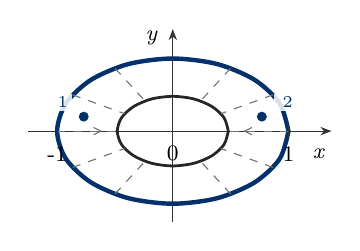
\begin{tikzpicture}[line join=round]
\draw[-{Stealth[length=4pt]},black!80] (0.720,-1.476) -- (4.572,-1.476);
\draw[-{Stealth[length=4pt]},black!80] (2.556,-2.628) -- (2.556,-0.180);
\draw[FAUblue,line width=1.6pt] plot[smooth,tension=0.5] coordinates {(4.025,-1.476) (3.913,-1.123) (3.594,-0.824) (3.119,-0.624) (2.556,-0.554) (1.993,-0.624) (1.518,-0.824) (1.199,-1.123) (1.087,-1.476) (1.199,-1.829) (1.518,-2.128) (1.993,-2.328) (2.556,-2.398) (3.119,-2.328) (3.594,-2.128) (3.913,-1.829) (4.025,-1.476)};
\draw[black!85,line width=1pt] plot[smooth,tension=0.5] coordinates {(3.261,-1.476) (3.207,-1.306) (3.054,-1.164) (2.826,-1.068) (2.556,-1.034) (2.286,-1.068) (2.058,-1.164) (1.905,-1.306) (1.851,-1.476) (1.905,-1.646) (2.058,-1.788) (2.286,-1.884) (2.556,-1.918) (2.826,-1.884) (3.054,-1.788) (3.207,-1.646) (3.261,-1.476)};
\draw[black!55,dashed] (3.290,-2.274) -- (2.909,-1.859);
\draw[black!55,dashed] (3.828,-1.937) -- (3.167,-1.697);
\draw[black!55,dashed] (4.025,-1.476) -- (3.261,-1.476);
\draw[black!55,dashed] (3.828,-1.015) -- (3.167,-1.255);
\draw[black!55,dashed] (3.290,-0.678) -- (2.909,-1.093);
\draw[black!55,dashed] (1.822,-0.678) -- (2.203,-1.093);
\draw[black!55,dashed] (1.284,-1.015) -- (1.945,-1.255);
\draw[black!55,dashed] (1.087,-1.476) -- (1.851,-1.476);
\draw[black!55,dashed] (1.284,-1.937) -- (1.945,-1.697);
\draw[black!55,dashed] (1.822,-2.274) -- (2.203,-1.859);
\draw[black!55,dashed] (3.467,-1.476) -- (3.636,-1.558);
\draw[black!55,dashed] (3.467,-1.476) -- (3.636,-1.394);
\draw[black!55,dashed] (1.645,-1.476) -- (1.476,-1.394);
\draw[black!55,dashed] (1.645,-1.476) -- (1.476,-1.558);
\fill[FAUblue] (1.425,-1.292) circle (0.063);
\node[anchor=east,text=FAUblue,fill=white,fill opacity=0.85,text opacity=1,inner sep=1pt,font=\footnotesize] at (1.281,-1.112) {ε\textsubscript{1}};
\fill[FAUblue] (3.687,-1.292) circle (0.063);
\node[anchor=west,text=FAUblue,fill=white,fill opacity=0.85,text opacity=1,inner sep=1pt,font=\footnotesize] at (3.831,-1.112) {ε\textsubscript{2}};
\node[anchor=east,inner sep=1pt,font=\footnotesize] at (4.536,-1.764) {\textit{x}};
\node[anchor=east,inner sep=1pt,font=\footnotesize] at (2.412,-0.288) {\textit{y}};
\draw[black!80] (1.087,-1.404) -- (1.087,-1.548);
\node[,inner sep=1pt,font=\footnotesize] at (1.087,-1.764) {-1};
\draw[black!80] (2.556,-1.404) -- (2.556,-1.548);
\node[,inner sep=1pt,font=\footnotesize] at (2.556,-1.764) {0};
\draw[black!80] (4.025,-1.404) -- (4.025,-1.548);
\node[,inner sep=1pt,font=\footnotesize] at (4.025,-1.764) {1};
\end{tikzpicture}\par\smallskip{\small\raggedright \textbf{Cross-section through the coaxial conductors.} The left and right half-annuli contain ε\textsubscript{1} and ε\textsubscript{2}. For positive \textit{U}\textsubscript{10}, the radial field points inward; the radial field lines run tangent to the straight dielectric interfaces.\par}\end{minipage}
\end{center}

\begin{keepsection}
\Needspace{7\baselineskip}
\subsection{9a: Sketch the electric field}

\Needspace{4\baselineskip}
Try first: identify the direction perpendicular to the conducting cylinders and compare it with the normal to each dielectric interface.

\nopagebreak[4]{\small\itshape Answers: see “Task 9: Electrostatics” under Answers at the end.}
\end{keepsection}

\begin{keepsection}
\Needspace{7\baselineskip}
\subsection{9b: Behaviour at the dielectric interface}

\Needspace{4\baselineskip}
Try first: at φ = \ensuremath{\pm}90°, name the surface normal and resolve the radial field into normal and tangential components.

\nopagebreak[4]{\small\itshape Answers: see “Task 9: Electrostatics” under Answers at the end.}
\end{keepsection}

\begin{keepsection}
\Needspace{7\baselineskip}
\subsection{9c: Mathematical approach for \textit{E}}

\Needspace{4\baselineskip}
Try first: write Laplace’s equation for a potential independent of φ and z, then use the two conductor potentials as boundary values.

\nopagebreak[4]{\small\itshape Answers: see “Task 9: Electrostatics” under Answers at the end.}
\end{keepsection}

\begin{keepsection}
\Needspace{6\baselineskip}
\subsection{9d: Relationship between \textit{D} and \textit{E}}

\Needspace{3\baselineskip}
Try first: use the constitutive law separately in each angular material region.

\nopagebreak[4]{\small\itshape Answers: see “Task 9: Electrostatics” under Answers at the end.}
\end{keepsection}

\begin{keepsection}
\Needspace{7\baselineskip}
\subsection{9e: Sign of charge on the outer cylinder}

\Needspace{4\baselineskip}
Try first: compare the specified potential of the outer conductor with the inner one and use the direction of \textit{E}.

\nopagebreak[4]{\small\itshape Answers: see “Task 9: Electrostatics” under Answers at the end.}
\end{keepsection}

\begin{keepsection}
\Needspace{7\baselineskip}
\subsection{9f: Find \textit{E} as a function of outer charge \textit{Q}}

\Needspace{4\baselineskip}
Try first: relate the field scale to the charge on the outer conductor by integrating \textit{D} over its inner cylindrical surface, split into two half-circumferences.

\nopagebreak[4]{\small\itshape Answers: see “Task 9: Electrostatics” under Answers at the end.}
\end{keepsection}

\begin{keepsection}
\Needspace{7\baselineskip}
\subsection{9g: Find \textit{U}\textsubscript{10} as a function of \textit{Q}}

\Needspace{4\baselineskip}
Try first: integrate the inward radial field between a and b, keeping the voltage reference \textit{U}\textsubscript{10} = φ\textsubscript{outer} \ensuremath{-} φ\textsubscript{inner} straight.

\nopagebreak[4]{\small\itshape Answers: see “Task 9: Electrostatics” under Answers at the end.}
\end{keepsection}

\begin{keepsection}
\Needspace{6\baselineskip}
\subsection{9h: Capacitance and numerical value}

\Needspace{3\baselineskip}
Try first: use \textit{C} = \textit{Q}/\textit{U}\textsubscript{10}, then substitute the two sector permittivities and dimensions.

\nopagebreak[4]{\small\itshape Answers: see “Task 9: Electrostatics” under Answers at the end.}
\end{keepsection}
\end{keepsection}


\clearpage
\section{Answers}
\begin{keepsection}\subsection{Task 9: Electrostatics}

\begin{workedbox}{9a \ensuremath{\cdot} Qualitative field}
\Needspace{10\baselineskip}
\begin{enumerate}
\item The metal cylinders are equipotentials. Away from the finite ends, the field meets each cylindrical conductor normally, so its direction is radial, along \textit{e}\textsubscript{ρ}.
\item The voltage is \textit{U}\textsubscript{10} = φ\textsubscript{outer} \ensuremath{-} φ\textsubscript{inner}. If \textit{U}\textsubscript{10} \ensuremath{>} 0, the outer conductor is at higher potential, so \textit{E} points inward (\ensuremath{-}\textit{e}\textsubscript{ρ}) from the outer cylinder toward the inner one. Reverse the arrows if \textit{U}\textsubscript{10} \ensuremath{<} 0.
\item Draw radial lines from radius \textit{b} to radius \textit{a}, with denser spacing near the inner cylinder because the field magnitude varies as 1/\textit{ρ}. Neglect end fringing as the ideal long-coax model requires.
\end{enumerate}
\end{workedbox}

\end{keepsection}
\begin{keepsection}\subsection{Task 9: Electrostatics}

\begin{workedbox}{9b \ensuremath{\cdot} Boundary conditions}
\Needspace{10\baselineskip}
\begin{enumerate}
\item \Needspace{5\baselineskip}
A constant-φ interface has normal \textit{n} = \ensuremath{\pm}\textit{e}\textsubscript{φ}. The radial field is perpendicular to that normal, so it lies tangent to the interface:

\begin{equation*}{E}_{\mathrm{n},1}\, =\, {E}_{\mathrm{n},2}\, =\, 0,\, \quad \, {E}_{\mathrm{t},1}\, =\, {E}_{\mathrm{t},2}\end{equation*}
\item \Needspace{6\baselineskip}
With no free charge on the dielectric boundary, the normal component of displacement is continuous; it is zero on both sides here. Tangential displacement need not be continuous and scales with each material permittivity:

\begin{equation*}{D}_{\mathrm{t},1}/{D}_{\mathrm{t},2}\, =\, ε_{1}/ε_{2}\end{equation*}
\item Thus \textit{E} crosses the angular boundary without a change in direction or magnitude. \textit{D} changes magnitude at the boundary in proportion to ε. The radial field lines run along the interface, rather than crossing it.
\end{enumerate}
\end{workedbox}

\end{keepsection}
\begin{keepsection}\subsection{Task 9: Electrostatics}

\begin{workedbox}{9c \ensuremath{\cdot} Radial solution}
\Needspace{10\baselineskip}
\begin{enumerate}
\item \Needspace{5\baselineskip}
The coaxial geometry and constant conductor potentials allow a z- and φ-independent potential in each sector. The cylindrical Laplace equation reduces to:

\Needspace{4\baselineskip}
\begin{equation*}(1/{ρ})\, \mathrm{d}/\mathrm{d}{ρ}({ρ}\, \mathrm{d}{V}/\mathrm{d}{ρ})\, =\, 0\end{equation*}

\begin{equation*}{V}({ρ})\, =\, \mathrm{A}\, \ln \, {ρ}\, +\, \mathrm{B}\end{equation*}
\item \Needspace{5\baselineskip}
Apply \textit{V}(\textit{a}) = φ\textsubscript{0} and \textit{V}(\textit{b}) = φ\textsubscript{1}. The same solution works in both sectors because their conductor boundary values are identical and the radial field is tangent to the interface:

\begin{equation*}{V}({ρ})\, =\, φ_{0}\, +\, {U}_{10}\, \ln ({ρ}/{a})/\ln ({b}/{a})\end{equation*}
\item \Needspace{4\baselineskip}
The electric field is the negative potential gradient:

\Needspace{5\baselineskip}
\begin{equation*}{E}({ρ})\, =\, -{U}_{10}/[{ρ}\, \ln ({b}/{a})]\, {e}_{ρ}\end{equation*}

The 1/\textit{ρ} dependence is required by cylindrical symmetry. Positive \textit{U}\textsubscript{10} gives the inward direction.
\end{enumerate}
\end{workedbox}

\end{keepsection}
\begin{keepsection}\subsection{Task 9: Electrostatics}

\begin{workedbox}{9d \ensuremath{\cdot} Piecewise permittivity}
\Needspace{6\baselineskip}
\begin{enumerate}
\item \Needspace{5\baselineskip}
For a linear, isotropic dielectric, \textit{D} = ε\textit{E}. The permittivity depends on which half-annulus contains the point:

\Needspace{4\baselineskip}
\begin{equation*}{D}({ρ},{φ})\, =\, ε_{1}{E}({ρ})\, \quad \, \text{for}\, 90°\, <\, {φ}\, <\, 270°\end{equation*}

\begin{equation*}{D}({ρ},{φ})\, =\, ε_{2}{E}({ρ})\, \quad \, \text{for}\, -90°\, <\, {φ}\, <\, 90°\end{equation*}
\item Because \textit{E} is the same on both sides of the radial interface, the displacement magnitudes differ by ε\textsubscript{1}/ε\textsubscript{2}. At φ = \ensuremath{\pm}90° the normal displacement remains zero and continuous.
\end{enumerate}
\end{workedbox}

\end{keepsection}
\begin{keepsection}\subsection{Task 9: Electrostatics}

\begin{workedbox}{9e \ensuremath{\cdot} Outer-conductor charge sign}
\Needspace{7\baselineskip}
\begin{enumerate}
\item For \textit{U}\textsubscript{10} \ensuremath{>} 0, the outer cylinder’s potential exceeds the inner cylinder’s. The field points from the outer conductor toward the inner conductor.
\item The normal from the metal into the dielectric at the outer cylinder’s inner wall is \ensuremath{-}\textit{e}\textsubscript{ρ}, parallel to \textit{E}. The conductor surface charge density there is \textit{D} \ensuremath{\cdot} (\ensuremath{-}\textit{e}\textsubscript{ρ}) \ensuremath{>} 0. Therefore the net charge on the outer cylinder is \textbf{positive}.
\end{enumerate}
\end{workedbox}

\end{keepsection}
\begin{keepsection}\subsection{Task 9: Electrostatics}

\begin{workedbox}{9f \ensuremath{\cdot} Charge fixes the field scale}
\Needspace{8\baselineskip}
\begin{enumerate}
\item \Needspace{6\baselineskip}
Let the inward field have magnitude \textit{K}/\textit{ρ}, so \textit{D} in sector i has magnitude ε\textsubscript{i}\textit{K}/\textit{ρ}. The normal from the outer metal into the gap is \ensuremath{-}\textit{e}\textsubscript{ρ}; its facing area is half the cylinder, π\textit{b l}, in each sector:

\begin{equation*}{Q}\, =\, (ε_{1}{K}/{b})(π{b\,l})\, +\, (ε_{2}{K}/{b})(π{b\,l})\end{equation*}
\item \Needspace{4\baselineskip}
Solve for the field constant and substitute into the radial field:

\Needspace{4\baselineskip}
\begin{equation*}{K}\, =\, {Q}/[π{l}(ε_{1}+ε_{2})]\end{equation*}

\Needspace{4\baselineskip}
\begin{equation*}{E}({ρ})\, =\, -{Q}/[π{l}(ε_{1}+ε_{2}){ρ}]\, {e}_{ρ}\end{equation*}

This is uniform in φ although \textit{D} is piecewise. The sign of Q sets the field direction.
\end{enumerate}
\end{workedbox}

\end{keepsection}
\begin{keepsection}\subsection{Task 9: Electrostatics}

\begin{workedbox}{9g \ensuremath{\cdot} Charge–voltage relation}
\Needspace{6\baselineskip}
\begin{enumerate}
\item \Needspace{4\baselineskip}
Because the field points inward, the outer-minus-inner voltage is \textit{U}\textsubscript{10} = \ensuremath{-}$\int_{\mathrm{a}}^{\mathrm{b}} $ \textit{E} \ensuremath{\cdot} \textit{e}\textsubscript{ρ} d\textit{ρ}:

\begin{equation*}{U}_{10}\, =\, {K}\, \int_{\mathrm{a}}^{\mathrm{b}} \, \mathrm{d}{ρ}/{ρ}\, =\, {K}\, \ln ({b}/{a})\end{equation*}
\item \Needspace{4\baselineskip}
Insert \textit{K} from 9f:

\Needspace{4\baselineskip}
\begin{equation*}{U}_{10}\, =\, [{Q}\, \ln ({b}/{a})]/[π{l}(ε_{1}+ε_{2})]\end{equation*}

Positive Q gives positive \textit{U}\textsubscript{10}, consistent with 9e.
\end{enumerate}
\end{workedbox}

\end{keepsection}
\begin{keepsection}\subsection{Task 9: Electrostatics}

\begin{workedbox}{9h \ensuremath{\cdot} Coaxial capacitance}
\Needspace{7\baselineskip}
\begin{enumerate}
\item \Needspace{5\baselineskip}
For this linear arrangement, capacitance is the charge magnitude per applied voltage. Cancel Q using 9g:

\begin{equation*}{C}\, =\, π{l}(ε_{1}+ε_{2})/\ln ({b}/{a})\end{equation*}
\item \Needspace{4\baselineskip}
With ε\textsubscript{1} = ε\textsubscript{0}, ε\textsubscript{2} = 3ε\textsubscript{0}, \textit{a} = 0.020 m, \textit{b} = 0.021 m and \textit{l} = 0.10 m:

\Needspace{4\baselineskip}
\begin{equation*}{C}\, =\, 4πε_{0}(0.10\, \mathrm{m})/\ln (0.021/0.020)\end{equation*}

\Needspace{5\baselineskip}
\begin{equation*}{C}\, \approx \, 2.28\, \times \, 10^{-10}\, \mathrm{F}\, =\, 228\, \text{pF}\end{equation*}

\textbf{Check:} a uniform ε\textsubscript{0} gap would have half this capacitance, since the mean permittivity here is 2ε\textsubscript{0}. The result is also positive and has units of farads.
\end{enumerate}
\end{workedbox}

\end{keepsection}

\vfill{\small Personal worked-solution guide based on the supplied EE1 Tutorial Task sheet, written in my own words; no tutorial text or figures are reproduced. Not an official FAU publication; check course details against current material. Made by \textbf{Thanate Amornjiraporn (Focus)}.}

\end{document}
